\documentclass[UTF8]{ctexart}

\usepackage{subfiles}  

%下面的语句, 引入你的头部设置文件
\usepackage{C:/phpStorm_proj/02_myself_ID_EGO/+100_latex_all_math_sel/myPreamble} 
%必须是绝对路径,才能让各个tex在单独编译时使用到

\title{文件名}


%---------------------------------


\begin{document}
	\tableofcontents % 生成目录
	\date{} % 若不写这句, 则默认也会渲染出日期, 所以我们要手动赋空值
	\maketitle  %这行代码, 让你前面的 title, author, date生效

	\part{正态分布 and 标准正态分布}
	
	\section{正态分布, normal distribution}
	
	正态分布, normal distribution, 直译过来就是``最常态下的分布", ``一般最常见的分布". \\
	正态分布, 是概率分布中最重要的分布. 在数学家眼里,它是远远高于其他分布的. 有很多其他的分布,比如对数正态分布、T分布、F分布, 都是直接由``正态分布"推导出来的. \\
	
	
	
	
	
	
	
	
	
	
	

\subsection{正态分布 - 概率密度函数 : $\boxed{
	\varphi (x)=\frac{1}{\sqrt[]{2\pi}\cdot \sigma}e^{-\frac{(x-\mu )^2}{2\sigma ^2}}
}$ }
	
	概率密度函数. 用小写的 $\varphi$ 表示. \\
	``正态分布" $N(\underset{\text{平均值}.}{\underbrace{\mu }},\underset{\sigma \text{是标准差.\ }\sigma ^2\text{是方差}}{\underbrace{\sigma ^2}})	$ 的概率函数是: 
	 $\boxed{
		\varphi (x)=\frac{1}{\sqrt[]{2\pi}\cdot \sigma}e^{-\frac{(x-\mu )^2}{2\sigma ^2}} \ (-\infty <x<+\infty )
	}$  \\
\vspace{1em} 

	记作: $\boxed{X \sim N(\mu ,\sigma ^2)}$   ← 称为: X服从``参数为$\mu$, $\sigma$的正态分布(或高斯分布)". \\	
	- 这里的 N, 就是正态分布 (Normal distribution) 的英文首字母.\\
	- $\mu$ 是 ``平均值" \\
	- $\sigma$ 是 ``标准差" \\
	- 注意: 概率函数公式里, 这第二个参数写的是$\sigma ^2$, 而不是$\sigma$! 所以, 比如对于N(1, 100)来说, 其 $\mu=1$,  $\sigma ^2=100$, 即$\sigma=10$. \\
	
	
\includegraphics[width=0.4\textwidth]{/0186.png} 
	
	
	
	
	\subsection{正态分布 - 累加函数 : $\boxed{
			F(x)=\frac{1}{\sqrt[]{2\pi}\cdot \sigma}\int_{-\infty}^x{\left[ e^{-\frac{(x-\mu )^2}{2\sigma ^2}} \right]}dx
		}$ }
	
	对``概率函数 f(x)"求积分, 其曲线下的阴影面积就是``累加函数 F(x)". 其面积=1. \\
	
	
	\begin{align*}  % 支持每行编号. 若不需要编号, 就用 align*环境
	&\underset{\text{累加函数}}{\underbrace{F(x)}}=\int_{}^{}{\underset{\text{概率函数}}{\underbrace{f(x)}}}dx\\
&=\int_{-\infty}^x{\left[ \frac{1}{\sqrt[]{2\pi}\cdot \sigma}e^{-\frac{(x-\mu )^2}{2\sigma ^2}} \right]}dx\\
&=\frac{1}{\sqrt[]{2\pi}\cdot \sigma}\int_{-\infty}^x{\left[ e^{-\frac{(x-\mu )^2}{2\sigma ^2}} \right]}dx
	\end{align*}



\vspace{1em} 
\subsection{正态分布(钟形曲线)的``概率函数"的性质}


\subsubsection{以 ``x=均值$\mu$" 为对称轴}

正态分布的``概率函数"曲线, 以 ``x=均值$\mu$" 为对称轴. 在此处, 函数的y值达到最大. 即此时 $y=\dfrac{1}{\sqrt[]{2\pi}\cdot \sigma}$ \\

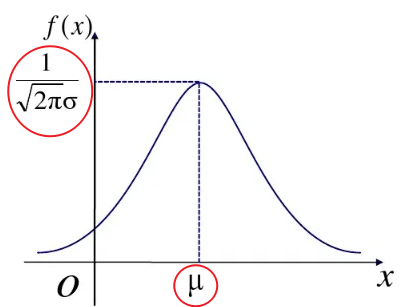
\includegraphics[width=0.35\textwidth]{/0187.png} \\

所以, 对称轴$\mu$, 能控制图像的``左右平移". \\




\subsubsection{以x轴为渐近线}
就是说, 曲线的两端, 无限接近于 y=0, 而不会掉落到 -y 领域上去.



\subsubsection{在 $x=\mu \pm \sigma $ 处有``拐点"}
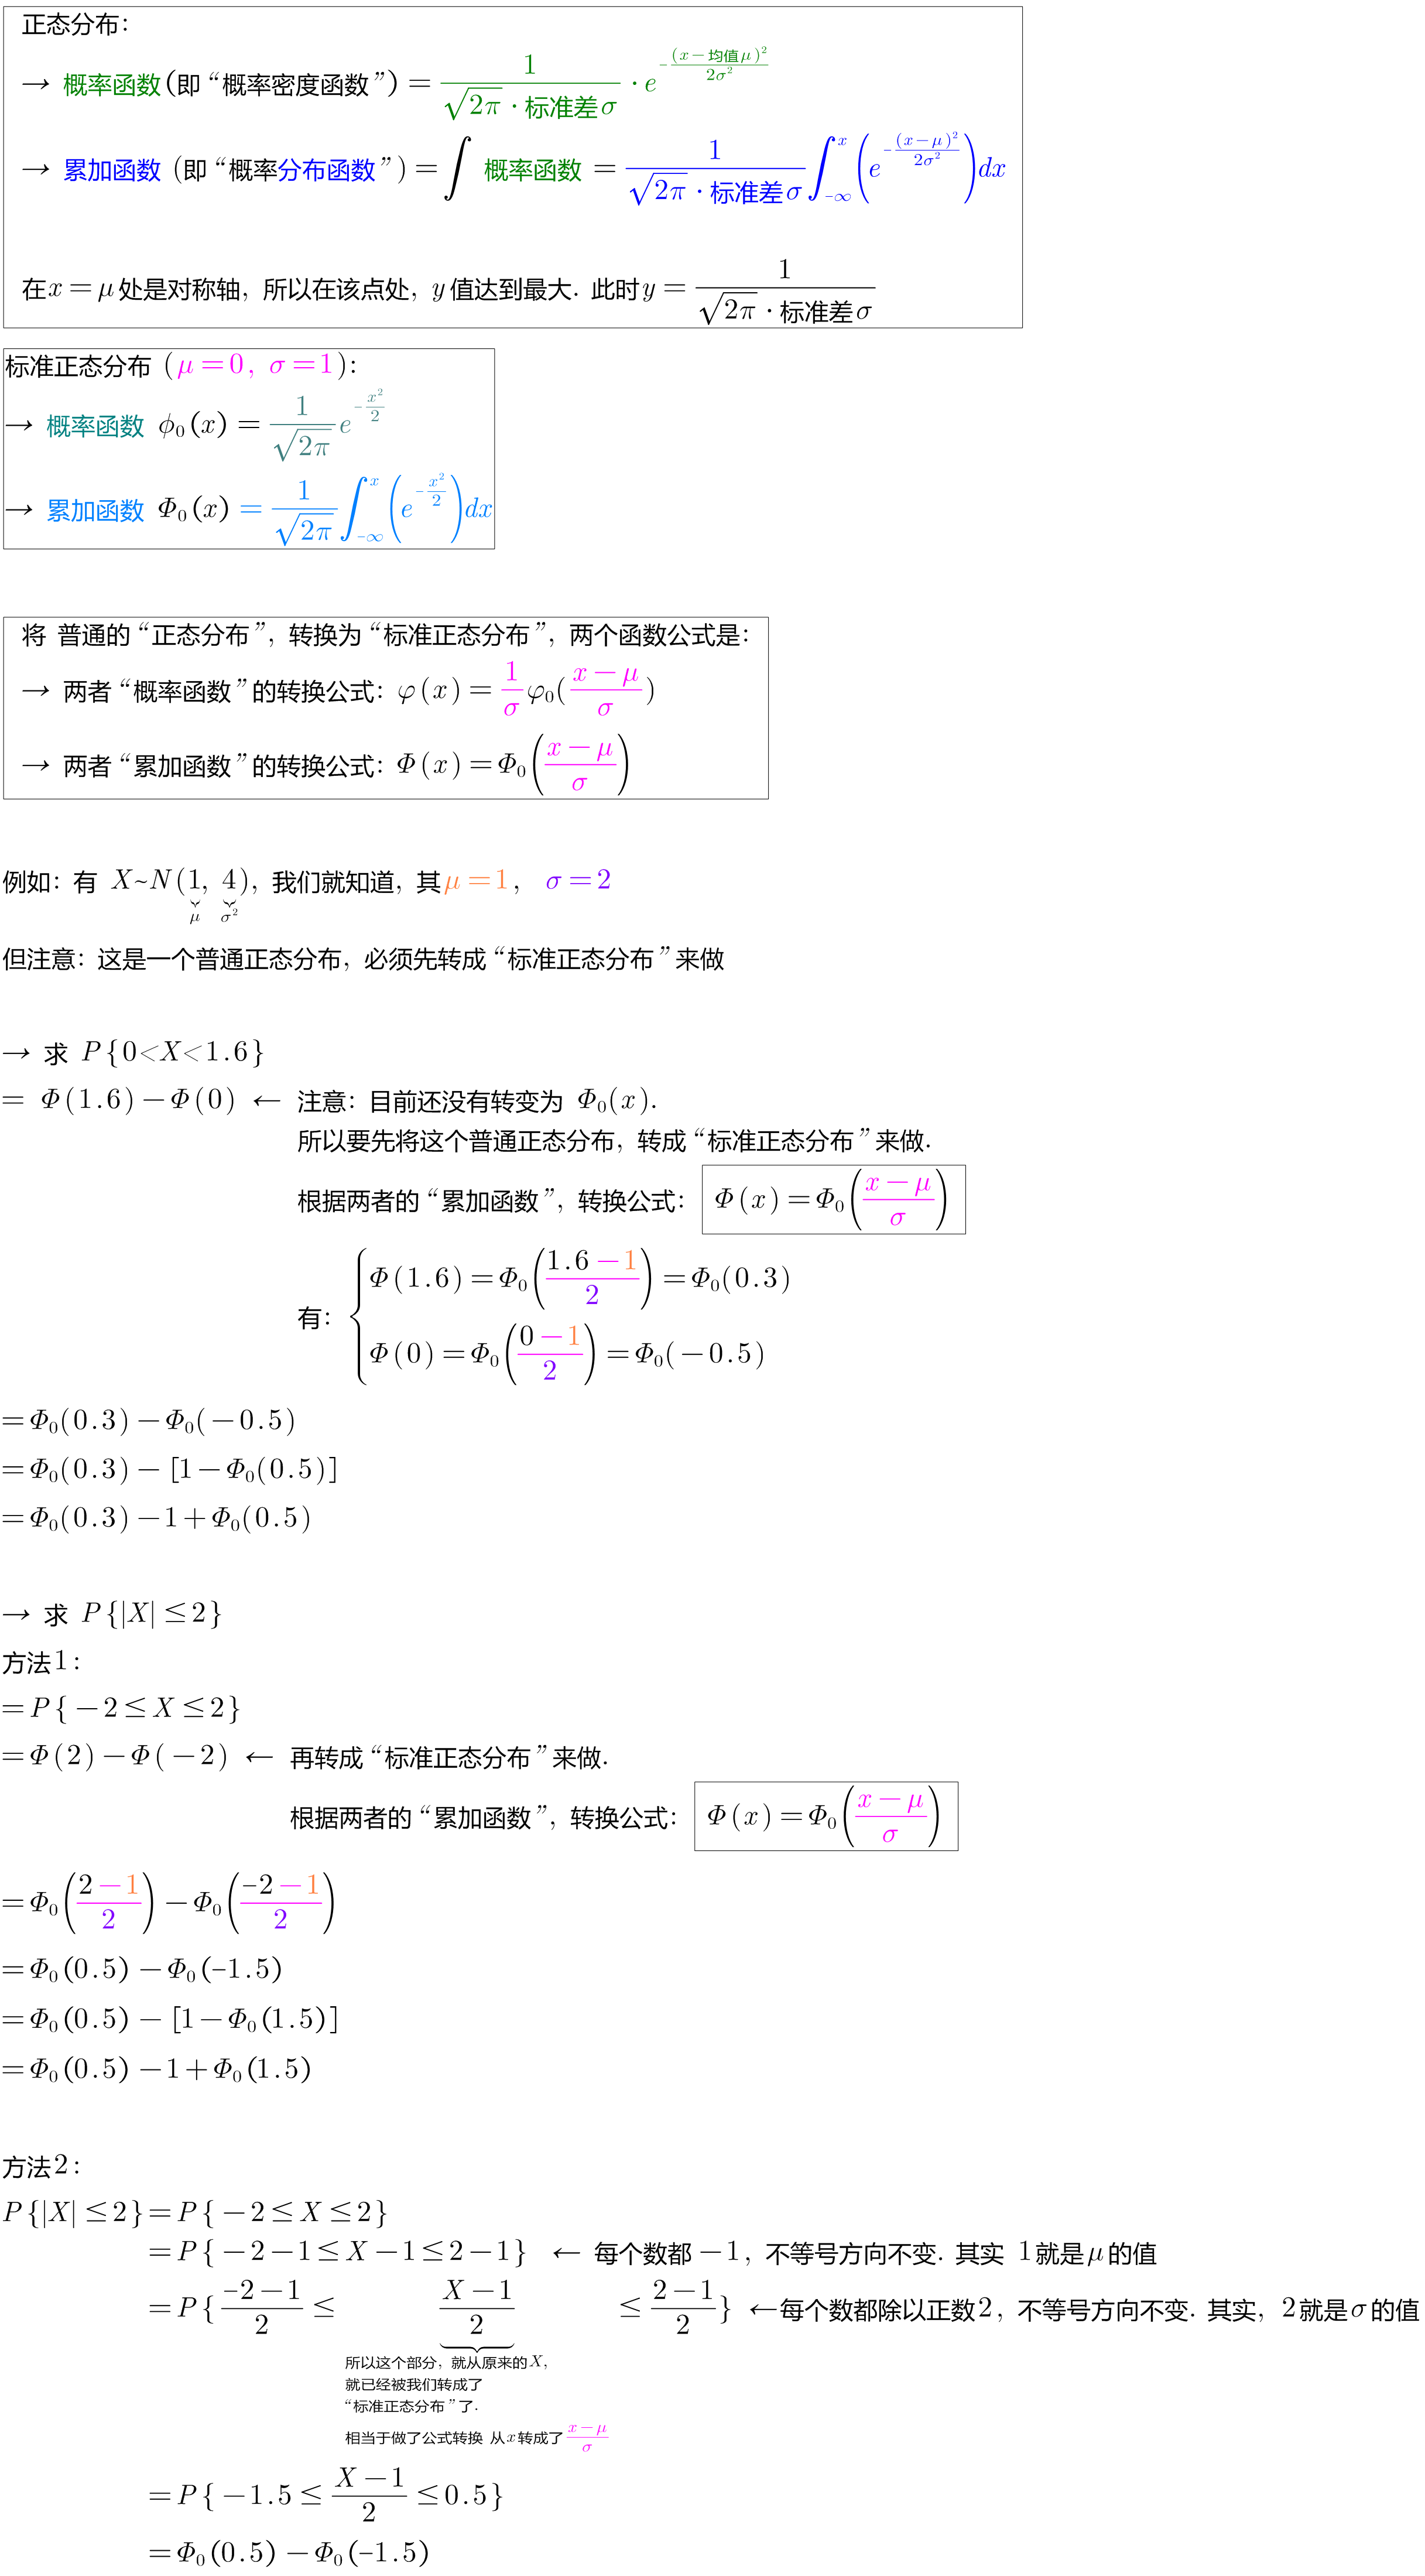
\includegraphics[width=0.7\textwidth]{/0188.png} 



\subsubsection{``$\sigma$ 标准差"参数, 控制图像的``矮胖"或``高瘦"}

→ 若$\sigma$ 变小: 因为 在x=μ处, y有最大值是 $ \dfrac{1} {\sqrt{2π} \cdot \sigma}$. 所以 当$\sigma$ 变小时, 分母变小, 则分数值就变大, 即y值变大, 所以图像会拉高, 变瘦高. \\
→ 若$\sigma$ 变大: 则最高点的y值变小, 图像会压低, 变矮胖. \\

但注意, 无论是变瘦高, 还是变矮胖, 曲线下的阴影面积, 始终是=1, 不变的! \\

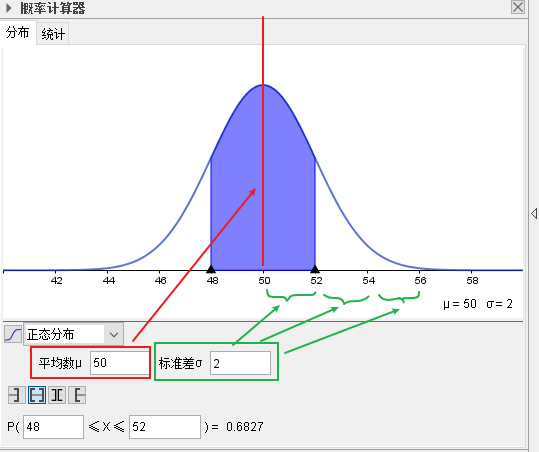
\includegraphics[width=0.65\textwidth]{/0189.png} 




~\\
\hrule
~\\



\section{标准正态分布 ← 即当 均值$\mu=0$, 标准差 $\sigma=1$ 时的``正态分布"}


\subsection{标准正态分布 - 概率函数 : $\boxed{
		\phi _0(x)=f\left( x \right) =\frac{1}{\sqrt[]{2\pi}}e^{-\frac{x^2}{2}}		
	}$}


我们把$\mu=0, \sigma=1$, 代入正态分布的 PDF 和 CDF 函数中, 就得到: \\

``标准正态分布"的``概率函数 PDF" (专门记作$\phi _0(x)$) :\\
$
\phi _0(x)=f\left( x \right) =\dfrac{1}{\sqrt[]{2\pi}\cdot \underset{=1}{\underbrace{\sigma }}}e^{-\frac{(x-\overset{=0}{\overbrace{\mu }})^2}{2\sigma ^2}}
=\dfrac{1}{\sqrt[]{2\pi}\cdot 1}e^{-\frac{(x-0)^2}{2\cdot 1^2}}
=\dfrac{1}{\sqrt[]{2\pi}}e^{-\frac{x^2}{2}}
$ \\

即: 
 $\boxed{
	\phi _0(x)=f\left( x \right) =\frac{1}{\sqrt[]{2\pi}}e^{-\frac{x^2}{2}}		
}$


\vspace{1em} 
\subsection{标准正态分布 - 累加函数 :  $\boxed{
		\varPhi _0(x)=F\left( x \right) =\frac{1}{\sqrt[]{2\pi}}\int_{-\infty}^x{\left[ e^{-\frac{x}{2}} \right]}dx
	}$}
	

``标准正态分布"的``累加函数 CDF" (专门记作$\varPhi _0(x)$) :
\begin{align*}  % 支持每行编号. 若不需要编号, 就用 align*环境
	\varPhi _0(x) &=F\left( x \right)\\
&=\frac{1}{\sqrt[]{2\pi}\cdot \underset{=1}{\underbrace{\sigma }}}\int_{-\infty}^x{\left[ e^{-\frac{(x-\overset{=0}{\overbrace{\mu }})^2}{2\sigma ^2}} \right]}dx\\
&=\frac{1}{\sqrt[]{2\pi}\cdot 1}\int_{-\infty}^x{\left[ e^{-\frac{(x-0)^2}{2\cdot 1^2}} \right]}dx\\
&=\frac{1}{\sqrt[]{2\pi}}\int_{-\infty}^x{\left[ e^{-\frac{x}{2}} \right]}dx  
\end{align*}

即: $\boxed{
	\varPhi _0(x)=F\left( x \right) =\frac{1}{\sqrt[]{2\pi}}\int_{-\infty}^x{\left[ e^{-\frac{x}{2}} \right]}dx
}$





\vspace{1em} 
\subsection{标准正态分布 的性质}

\subsubsection{因为它的 $\mu=0$, 所以它的函数曲线, 关于 x=0 对称, 即y轴是对称轴.}

所以它就是个偶函数.  有: \\
- 概率函数 $ \varphi_0(x) = \varphi_0(-x) $   ← 我们在下标处加个0, 来表示它是``标准"的正态分布函数的 ``概率函数"或``累加函数". \\

- 其``累加函数"有: $\boxed{\varPhi _0(-x)=1-\varPhi _0(x)}$ ← 这个公式很重要! \\
比如 : $\varPhi _0(-4)=1-\varPhi _0(4)$ \\

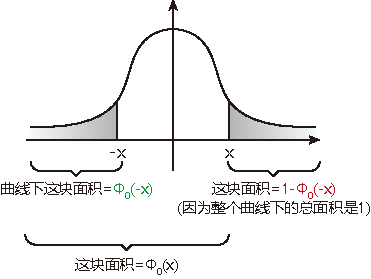
\includegraphics[width=0.5\textwidth]{/0190.pdf} \\
	
	
\begin{myEnvSample}
	\begin{align*}  % 支持每行编号. 若不需要编号, 就用 align*环境
	\text{求} \ P\{|x|\leq 1.96\} &=P\{-1.96\leq X\leq 1.96\}\\
&=\varPhi _0(1.96)-\underset{=1-\varPhi _0(1.96)}{\underbrace{\varPhi _0(-1.96)}}\\
&=\varPhi _0(1.96)-1+\varPhi _0(1.96)\\
&=2\varPhi _0(1.96)-1
	\end{align*}

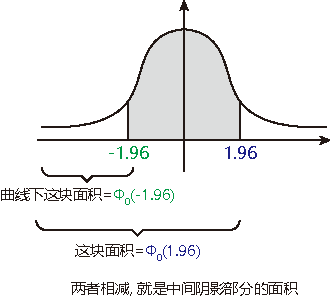
\includegraphics[width=0.5\textwidth]{/0191.pdf} 
\end{myEnvSample}	






\subsubsection{对于 $ x \geq 5$ 的y值, 已经非常靠近y=0了}

正态分布的值, 怎么算? --- 查表. \\
一般, 书上给出的都是``标准正态分布"的表. 所以如果你是普通的``正态分布", 必须先把它转成``标准正态分布", 再来查表. \\

并且, 表的范围, 只给出了 $ 0 \leq x < 5$  的值. \textbf{因为对于$ x \geq 5$ 的值, 此时的曲线高度, 即y值, 已经非常靠近y=0了. 所以我们就可以认为: 对于$ x \geq 5$ 的 标准正态分布的``概率函数 $ \varphi_0(x)$"的y值, 都=0.} \\


同样, 来看累加函数 CDF: \\
对于 $ x \geq 5$ 时, 其位置已经非常靠近整个曲线的右端末尾了, 而整个函数曲线下的面积也就=1, 所以, 在 $ x \geq 5$  处的``累加函数$ \Phi_0(x)$", 其值我们就可以认为是1. \\

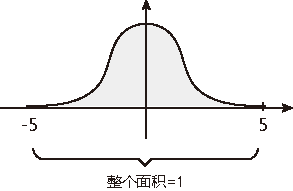
\includegraphics[width=0.45\textwidth]{/0192.pdf}  \\

即: \\
\begin{tabular}{|l|l|l|}
	\hline
	标准正态分布 & 概率函数 $\varphi _0(x)$  & 累加函数 $\Phi _0(x)$ \\
	\hline
	当 $x \leq -5$ 时 & $y \approx 0$ & $y \approx 0$\\
	\hline
	当 $x \geq 5$ 时 & $y \approx 0$ & $y \approx 1$\\
	\hline
\end{tabular} \\








\section{普通的``正态分布", 怎样转化成``标准正态分布"?}

\subsection{``概率函数"的转化公式是: $\boxed{
	\varphi (x)=\frac{1}{\sigma}\cdot \varphi _0(\frac{x-\mu}{\sigma})
	}$}

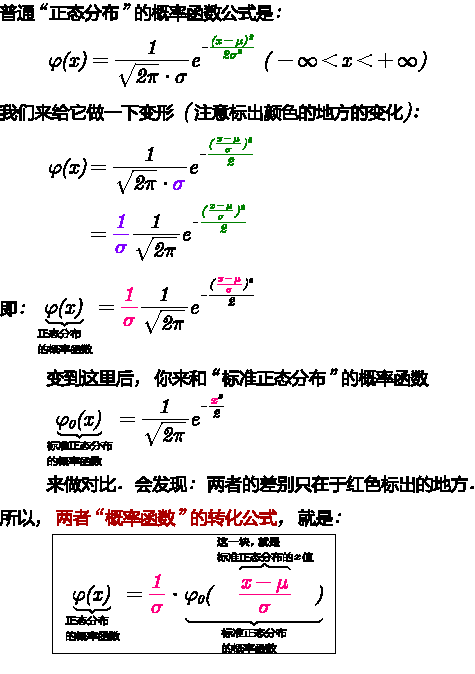
\includegraphics[width=0.6\textwidth]{/0193.pdf} \\




\subsection{``累加函数"的转化公式是: $\boxed{\varPhi (x)=\varPhi _0(\frac{x-\mu}{\sigma})	}$}

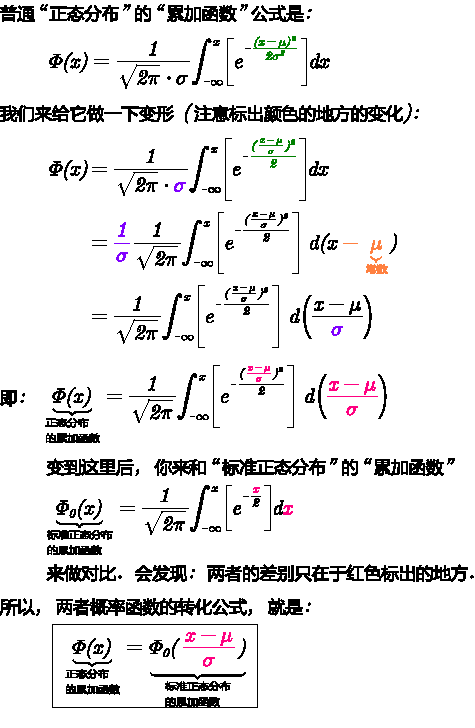
\includegraphics[width=0.6\textwidth]{/0194.pdf} \\



\begin{myEnvSample}
有 $X \sim N(1,4)$, 即 $\mu=1, \ \sigma^2=4,\ \sigma=2$ \\
到注意: 这只是一个普通的正态分布, 我们必须先把它转成``标准正态分布"再来做. \\

→ 求 $P\{0<X<1.6\} =\varPhi (1.6)-\varPhi (0)$ \\
先把这个累加函数$\Phi (x)$ (正态分布的), 转成$\Phi_0 (x)$ (标准正态分布的). 套用转化公式, 就有: \\
$	\varPhi (1.6)=\varPhi _0\left( \frac{x-\mu}{\sigma} \right) =\varPhi _0\left( \frac{1.6-1}{2} \right) =\varPhi _0(0.3)$ \\
$	\varPhi (0)=\varPhi _0\left( \frac{x-\mu}{\sigma} \right) =\varPhi _0\left( \frac{0-1}{2} \right) =\varPhi _0(-0.5)$ \\

所以回到原题, $
\varPhi (1.6)-\varPhi (0)=\varPhi _0(0.3)-\underset{=1-\varPhi _0(0.5)}{\underbrace{\varPhi _0(-0.5)}}
$ \\

→ 求 $P\left\{ |X|\leq 2 \right\} $ \\
方法1: 
\begin{align*}  % 支持每行编号. 若不需要编号, 就用 align*环境
	P\left\{ |X|\leq 2 \right\} &=P\left\{ -2\leq X\leq 2 \right\}\\
&=\varPhi \left( 2 \right) -\varPhi \left( -2 \right) \ \gets \text{转成} \text{``标准正态分布"}”\text{的累加函数}\\
&=\varPhi _0\left( \frac{2-\overset{\mu}{\overbrace{1}}}{\underset{\sigma}{\underbrace{1}}} \right) -\varPhi _0\left( \frac{-2-1}{1} \right)\\
&=\varPhi _0\left( 0.5 \right) -\varPhi _0\left( -1.5 \right)\\
&=\varPhi _0\left( 0.5 \right) -\left[ 1-\varPhi _0\left( 1.5 \right) \right]
\end{align*} 

方法2: 
\begin{align*}  % 支持每行编号. 若不需要编号, 就用 align*环境
	P\left\{ |X|\leq 2 \right\}
&=P\left\{ -2\leq X\leq 2 \right\}\\
&=P\left\{ \left( -2-1 \right) \leq \left( X-1 \right) \leq \left( 2-1 \right) \right\} \ \gets \text{对}X\text{左中右,同时减去}\mu \text{值}1\\
&=P\left\{ \frac{-2-1}{2}\leq \frac{X-\overset{\mu}{\overbrace{1}}}{\underset{\sigma}{\underbrace{2}}}\leq \frac{2-1}{2} \right\} \ \gets \text{对}X\text{左中右,同时除以}\sigma \text{值}2\\
&\text{注意,现在中间的}\frac{X-1}{2},\text{就已经被我们转化成了``标准正态分布"的x形式了},\\
&\text{即从}x\text{转成了}\frac{x-\mu}{\sigma}\\
&=P\left\{ -1.5\leq \frac{X-1}{2}\leq 0.5 \right\}\\
&=\varPhi _0\left( 0.5 \right) -\varPhi _0\left( -1.5 \right)
\end{align*}

\end{myEnvSample}
\vspace{1em} 




\begin{myEnvSample}
飞船零件, 尺寸符合``正态分布" $X\sim N\left( \underset{\mu}{\underbrace{50}},\underset{\sigma ^2}{\underbrace{1}} \right) $, 即 $\sigma=1$ \\
其尺寸只有在 $50 \pm 1$ 时, 才是合格的. \\

那么问:  \\
→ 生产出的单个飞船零件, 合格概率是? 
\begin{align*}  % 支持每行编号. 若不需要编号, 就用 align*环境
	P\left\{ 49\leq X\leq 51 \right\} 
&=\varPhi \left( 51 \right) -\varPhi \left( 49 \right)\\
&=\varPhi _0\left( \frac{51-\overset{\mu}{\overbrace{50}}}{\underset{\sigma}{\underbrace{1}}} \right) -\varPhi _0\left( \frac{49-50}{1} \right)\\
&=\varPhi _0\left( 1 \right) -\varPhi _0\left( -1 \right)\\
&=\varPhi _0\left( 1 \right) -\left( 1-\varPhi _0\left( 1 \right) \right) =0.68269 
\end{align*}

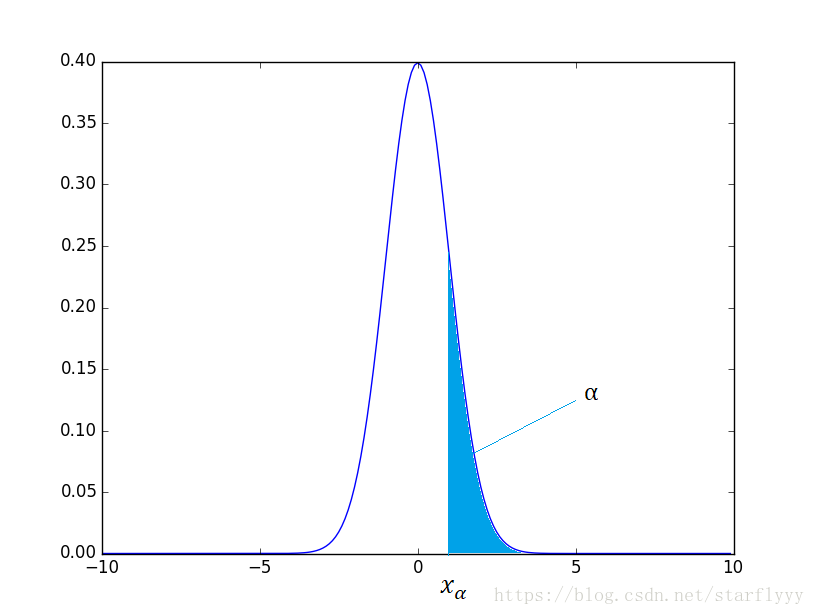
\includegraphics[width=0.5\textwidth]{/0195.png} \\



→ 重复抽检3次, 至少有1个零件是合格的概率?
\begin{align*}  % 支持每行编号. 若不需要编号, 就用 align*环境
	P\underset{\text{我们令}Y\text{表示合格品的数量}}{\underbrace{\left\{ Y\ge 1 \right\} }}
	&=1-\underset{\text{所抽的3件都不合格\ 的概率}}{\underbrace{P\left\{ Y=0 \right\} }}\\
&=1-\left( 1-\underset{\text{单个产品的合格率}}{\underbrace{0.6827}} \right) ^3=0.968054
\end{align*}
\end{myEnvSample}
\vspace{1em} 




\begin{myEnvSample}

\end{myEnvSample}




\end{document}